\documentclass[11pt]{article}
\usepackage{amsmath, amssymb}
\usepackage{geometry} % see geometry.pdf on how to lay out the page. There's lots.
\geometry{a4paper} % or letter or a5paper or ... etc
\usepackage{graphicx}
% \geometry{landscape} % rotated page geometry
% See the ``Article customise'' template for come common customisations
\usepackage[style=phys,
citestyle=phys]{biblatex}
\addbibresource{van_vleck_memo_A.bib}

\usepackage{listings}

\title{Implementation of Van Vleck Correction for the MWA}
\author{Pyxie Star}
% delete this line to display the current date
\renewcommand{\Re}{\operatorname{Re}}
\renewcommand{\Im}{\operatorname{Im}}

%%% BEGIN DOCUMENT
\begin{document}

\maketitle
% \section{Introduction}
\paragraph{}Quantization occurs in multiple stages of the MWA digital signal pathway and introduces small-scale nonlinearity into the data. This nonlinearity interacts with spectral structure, particularly the periodic response of the 2-stage polyphase filter banks, to result in non-negligible calibration errors. In order to achieve the sensitivity necessary for an EOR detection, the instrument spectral structure calibration must be accurate to an order of $10^{-5}$. Due to the interactions between the small-scale quantization effects and the PFB structure, residual periodic response is left in the data after calibration and contaminates the power spectra. In order to cleanly remove the instrument response through calibration, we must first address the nonlinear artifacts from quantization.

\paragraph{}
Data products from the MWA are complex visibilities, that is, cross-correlations between each antenna and auto-correlations of each antenna with itself. The nonlinearity of quantization effects requires that each visibility receive a unique correction. With 8256 antenna combinations from MWA II, 768 frequencies, and 4 polarizations, this results in $~10^9$ computations for each 2 minute observation taken at 0.5 seconds. Thus implementations of a correction for these nonlinearities must take computational efficiency into consideration.

\paragraph{}Formulae for correcting these artifacts with a Van Vleck correction were presented in \cite{VV}. An implementation of the correction has been written into \texttt{pyuvdata} as an option when reading raw MWA correlator output files. This memo describes MWA quantization, re-derives the correction formulae, and discusses the implementation.

\section{MWA Quantization}
\paragraph{}
Quantization occurs in multiple stages of the MWA digital signal pathway, with the ultimate stage being a 4 + 4 bit quantization immediately before correlation. It is this final quantization that the current implementation of the Van Vleck correction addresses. A second implementation of the Van Vleck correction is in development to address a previous quantization stage in the correlator polyphase filter bank (PFB). These quantization stages are described below in a summary of the digital signal pathway.
\paragraph{}
The analog signal from a tile is attenuated to $\pm1$ Volt, and a bandpass is applied to limit the frequency range to 80-300 MHz. This signal then goes to a digital receiver, described in \cite{rec}, where it is sampled at 655.36 MHz and quantized to 8-bit values. The quantized data is then cast from real to complex, and also channelized into 256 1.28 MHz channels by the 'coarse' PFB. The coarse PFB has an 8 tap subfilter followed by a 512 point FFT, and functions as follows. A Kaiser windowing function is applied to 4096 data samples. The 4096 windowed samples are split into 8 'phases' of 512 samples each, which are summed to result in 512 inputs to the FFT. The FFT outputs 256 complex values each consisting of a 16-bit real and 16-bit imaginary pair. Since each frequency channel is complex, that is, carrying two sampled values, the sampling rate is halved to 327.68 MHz. The incoming data is then shifted by 512 samples and the PFB procedure applied to this next grouping. After the FFT, a gain is applied to the data, and another quantization occurs, taking the 16-bit real, 16-bit imaginary pair to a 5-bit real, 5-bit imaginary pair. For each observing session, some subset of 24 coarse channels is chosen and sent to the correlator. 
\paragraph{}
The MWA correlator \cite{corr} has two stages: a 'fine' PFB which further channelizes the data, and a cross-multiply and accumulate module to perform the correlations. The fine PFB  has a 12-tap subfilter that applies a Hanning window to the data stream, followed by a 128-point FFT. Outputs of the fine PFB are quantized to 4-bit real, 4-bit imaginary pairs, and these integers are cast to floats for input into the correlator cross-multiply. As discussed in \cite{pfb}, an asymmetric 8 + 8 bit re-quantization occurs in the fine PFB between the subfilter and the FFT. This asymmetric rounding will be addressed by the second stage of the Van Vleck correction.

\section{4-bit Van Vleck Correction}
\begin{figure}
\centering{}
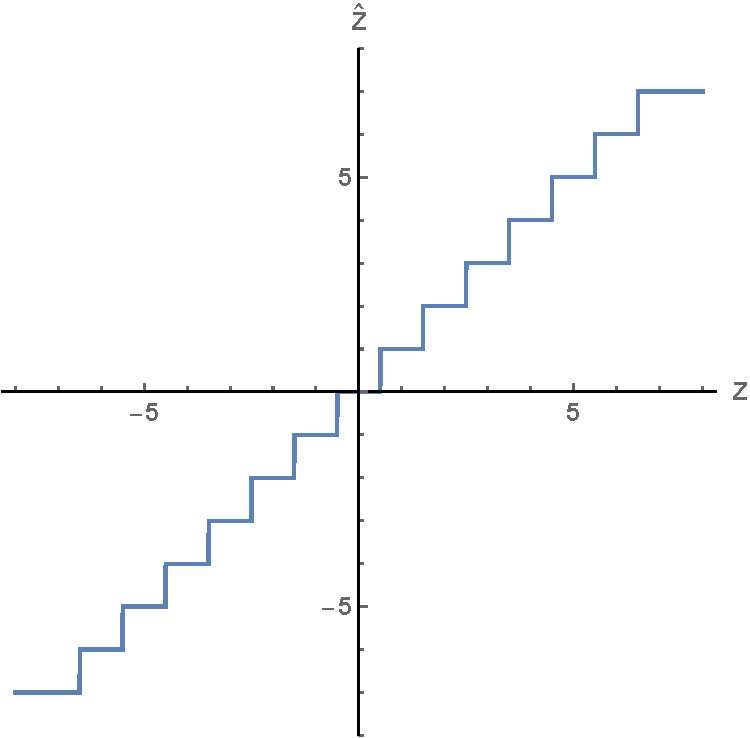
\includegraphics[width=80mm]{quant.pdf}
\caption{The 4-bit quantization pattern of the MWA.\label{quant}}
\end{figure}

\paragraph{}
The final 4-bit quantization in the correlator is assumed to have a dominant contribution to nonlinear artifacts, and so is addressed in the initial Van Vleck implementation. For the correction model, we treat the values going into the 4-bit quantization as being sampled from an analog signal. The correction can be understood as mapping the estimated standard deviation of the distribution of a quantized signal to the estimated standard deviation of the initial analog signal. To apply the correction using visibilities, we relate the autocorrelations $V_{ii}$ and the crosscorrelations $V_{ij}$ to the statistical distributions of the signal. Our signals are complex, and as shown in the following sections, we are interested in the underlying statistical distribution of the real and imaginary parts of these signals. In \S \ref{autos1} we lay out the relationship between an analog autocorrelation $V_{11}$ and the standard deviation of the analog signal $\sigma_{t_1}$. Then in \S \ref{autos2}, the quantization pattern is used to relate an autocorrelation of quantized values $\hat V_{11}$ to $\sigma_{t_1}$, and thus to $V_{11}$. This relation provides the correction for autocorrelations. A similar analysis is performed in \S \ref{cross1}, relating the real and imaginary parts of an analog crosscorrelation $V_{12}$ to the covariance between the real or imaginary parts of two signals $E[X_1X_2]$ and $E[X_1Y_2]$. The Van Vleck correction maps $E[X_1X_2]$ and $E[X_1Y_2]$ to the corresponding quantized $E[\hat X_1\hat X_2]$ and $ E[\hat X_1\hat Y_2]$ and thus to $\hat V_{12}$, as is shown in  \S \ref{cross2}.

\subsection{Analog autocorrelations}\label{autos1}
\paragraph{}
In the case of an analog signal which is sampled without quantization, let the correlator input from antenna 1 (with arbitrary polarization) be $Z_1$, where $Z_1$ is the sum of a sky signal and receiver noise: $Z_1=S_1+ N_1$. Both $S_1$ and $N_1$ are complex circular Gaussian random variables. That is, the real and imaginary parts are each Gaussian distributed with zero mean, and are uncorrelated with each other. Alternatively, we can think of this as there being no preferred phase in either the sky signal or in the receiver noise. We additionally assume that $Z_1$ itself is a complex circular Gaussian random variable, which might require assumptions about the lack of correlation between sky signal and instrument noise (see Appendix \ref{ccrv}). The real and imaginary parts of $Z_1$ are drawn from a distribution with standard deviation $\sigma_{t_1}$. As shown below, the autocorrelation $V_{11}$ gives an estimate of $\sigma_{t_1}$. We can write $Z_1$ in terms of its real and imaginary components as 
\begin{equation}
Z_1=X_1+iY_1,
\end{equation}
where $X_1$ and $Y_1$ are zero-mean Gaussian distributed. The autocorrelation is calculated by summing $N$ samples of $Z_1Z_1^*$. That is,
\begin{align}
V_{11} &= \sum_{j=1}^N Z_{1_j}Z_{1_j}^*\\
&= \sum_{j=1}^N (X_{1_j} + iY_{1_j})(X_{1_j}-iY_{1_j})\\
&= \sum_{j=1}^N X_{1_j}^2 + \sum_{j=1}^N Y_{1_j}^2.
\end{align}
In the limit of large $N$, the sums can be used to approximate the second moments of $X_1$ and $Y_1$ with
\begin{align}
\frac{1}{N}\sum_{j=1}^N X_{1_j}^2 &\rightarrow E[X_1^2],\\
\frac{1}{N}\sum_{j=1}^N Y_{1_j}^2 &\rightarrow E[Y_1^2];
\end{align}
where, since $X_1$ and $Y_1$ are zero-mean Gaussian, $E[X_1^2] =\sigma_{x_1}^2$ and $E[Y_1^2]=\sigma_{y_1}^2$. Additionally, $X_1$ and $Y_1$ have the same distribution, so $\sigma_{x_1}=\sigma_{y_1}$. Thus, with sufficiently large $N$, we can write the autocorrelation $V_{11}$ in terms of $\sigma_{x_1}$, an estimate of the true analog standard deviation $\sigma_{t_1}$:
\begin{align}
\frac{V_{11}}{N}&=\frac{1}{N}\sum_{j=1}^N X_{1_j}^2+\frac{1}{N}\sum_{j=1}^N Y_{1_j}^2\\
&=\sigma_{x_1}^2 + \sigma_{y_1}^2\\
&= 2\sigma_{x_1}^2\\
&\simeq 2\sigma_{t_1}^2
\end{align}
For later use in the Van Vleck correction, it is convenient to rewrite the above expression in the form
\begin{equation}\label{auto}
\sqrt{V_{11}/2N}=\sigma_{x_1}.
\end{equation}

\subsection{Autocorrelation correction}\label{autos2}
The 4-bit quantization sorts the real and imaginary parts of the analog signal measured by antenna 1, $X_1$ and $Y_1$, into integer bins ranging inclusively from -7 to 7, as shown in figure~\ref{quant}. The autocorrelation $\hat V_{11}$ of these quantized samples is calculated as
\begin{align}
\hat V_{11} &= \sum_{j=1}^N \hat Z_{1_j} \hat Z_{1_j}^*\\
&= \sum_{j=1}^N \hat X_{1_j}^2 + \sum_{j=1}^N \hat Y_{1_j}^2.
\end{align}
Again, we use the large $N$ limit to write
\begin{align}
\frac{\hat V_{11}}{N} &\rightarrow E[\hat X_1^2] + E[\hat Y_1^2]\\
&= 2 E[\hat X_1^2],
\end{align}
where, in the last line, we have used the fact that $\hat X_1$ and $\hat Y_1$ have the same distribution, thus $E[\hat X_1^2] = E[\hat Y_1^2]$. Writing in a convenient form gives 
\begin{equation}\label{autohat}
\hat V_{11}/2N\simeq E[\hat X_1^2].
\end{equation}

\paragraph{}
As outlined in \cite{VV}, we use the quantization pattern to relate $E[\hat X_1^2]$ to $ \sigma_{x_1}$, and thus $\hat V_{11}$ to $V_{11}$, as follows. The expectation value $E[\hat X_1^2]$ is defined
\begin{equation}
\begin{split}
E[\hat X_1^2]=&0^2\cdot P(\hat X_1 = 0) +(-1)^2\cdot P(\hat X_1 = -1)+1^2\cdot P(\hat X_1 = 1)+\cdot\cdot\cdot\\
&+(-7)^2\cdot P(\hat X_1 = -7)+7^2\cdot P(\hat X_1 = 7).
\end{split}
\end{equation}
The probability of $\hat X_1$ taking a particular quantized value is equal to the probability of $X_1$ falling into the corresponding quantization bin. Thus the expectation value can be written
\begin{equation}
\begin{split}
E[\hat X_1^2]=&0^2\cdot P(-0.5<X_1<0.5) +(-1)^2\cdot P(-1.5<X_1<-0.5)+1^2\cdot P(0.5<X_1<1.5)+\cdot\cdot\cdot\\
&+(-7)^2\cdot P(X_1<-6.5)+7^2\cdot P(X_1>6.5).
\end{split}
\end{equation}
Taking advantage of the symmetries of both the distribution of $X_1$ and the quantization bins, 
\begin{equation}
\begin{split}
E[\hat X_1^2]=&0^2\cdot P(-0.5<X_1<0.5)+1^2\cdot[P(-1.5<X_1<1.5)-P(-0.5<X_1<0.5)]+\cdot\cdot\cdot\\
&+7^2\cdot[1-P(-6.5<X_1<6.5)].
\end{split}
\end{equation}
With $X_1$ drawn from a zero-mean Gaussian distribution with $\sigma_{t_1}$, the probability that $X_1\in[-a,a]$,
\begin{equation}
P(X_1\in[-a,a])=\textrm{erf}\left(\frac{a}{\sigma_{t_1}\sqrt{2}}\right).
\end{equation}
Substituting this probability and combining terms gives the compact expression
\begin{align}
E[\hat X_1^2]=&0^2\cdot\textrm{erf}\left(\frac{0.5}{\sigma_{t_1}\sqrt{2}}\right)+1^2\cdot\left[\textrm{erf}\left(\frac{1.5}{\sigma_{t_1}\sqrt{2}}\right)-\textrm{erf}\left(\frac{0.5}{\sigma_{t_1}\sqrt{2}}\right)\right]+\cdot\cdot\cdot+7^2\cdot\left[1-\textrm{erf}\left(\frac{6.5}{\sigma_{t_1}\sqrt{2}}\right)\right]\nonumber\\
=&(-1)\textrm{erf}\left(\frac{0.5}{\sigma_{t_1}\sqrt{2}}\right)+(-3)\textrm{erf}\left(\frac{1.5}{\sigma_{t_1}\sqrt{2}}\right)+\cdot\cdot\cdot+(-13)\textrm{erf}\left(\frac{6.5}{\sigma_{t_1}\sqrt{2}}\right)+7^2\nonumber\\
=&7^2-\sum_{k=0}^6(2k+1)\textrm{erf}\left(\frac{k+0.5}{\sigma_{t_1}\sqrt{2}}\right)\nonumber\\
\simeq&7^2-\sum_{k=0}^6(2k+1)\textrm{erf}\left(\frac{k+0.5}{\sigma_{x_1}\sqrt{2}}\right).
\end{align}
Using equations \eqref{auto} and \eqref{autohat}, and taking the square root of both sides, the above relation can be written in terms of $V_{11}$ and $\hat V_{11}$ as
\begin{equation}\label{autocorr}
\boxed{\sqrt{\hat V_{11}/2N} \simeq \left[7^2-\sum_{k=0}^6(2k+1)\textrm{erf}\left(\frac{k+0.5}{\sqrt{V_{11}/2N}\sqrt{2}}\right)\right]^{1/2}. }
\end{equation}
Thus by inverting the above equation, we can obtain an estimate of the autocorrelation of analog values $V_{11}$ from the corresponding autocorrelation of quantized values $\hat V_{11}$. Through calculating $V_{11}$ we obtain $\sigma_{x_1}$, and thus can estimate the standard deviation $\sigma_{t_1}$ of the analog values, which will be useful in the correction for crosscorrelations.

\subsection{Analog crosscorrelations}\label{cross1}
A similar analysis can be done for the analog crosscorrelation between antenna 1 and antenna 2, $V_{12}$, which is calculated by summing $N$ samples of $Z_1Z_2^*$ so that
\begin{align}
 V_{12}&=\sum_{j=1}^N Z_{1_j}Z_{2_j}^*\\
 &=\sum_{j=1}^N(X_{1_j} + iY_{1_j})(X_{2_j} -iY_{2_j})\\
 &=\sum_{j=1}^N(X_{1_j} X_{2_j}  + Y_{1_j}Y_{2_j} +i Y_{1_j}X_{2_j} -i X_{1_j} Y_{2_j}).
 \end{align}
The limit of large N can again be taken to give, for any combination of $X_1, Y_1$ with $X_2, Y_2$:
\begin{equation}
\frac{1}{N}\sum_{j=1}^N X_{1_j}X_{2_j} \rightarrow E[X_1X_2].
\end{equation}
Thus in this limit, the crosscorrelation
\begin{align}
\frac{V_{12}}{N}&\rightarrow E[X_{1} X_{2}]  + E[Y_{1}Y_{2}] +i E[Y_{1}X_{2}] -i E[X_{1} Y_{2}]\\
&=2E[X_{1} X_{2}]  + 2iE[Y_{1}X_{2}],
\end{align}
where the last step has used the following relations for circular complex random variables:
\begin{align}
E[X_{1} X_{2}] &=E[Y_{1}Y_{2}] \\
E[Y_{1}X_{2}] &=-E[X_{1} Y_{2}]
\end{align}
Rewriting in terms of the real and imaginary parts of $V_{12}$ gives
\begin{equation}\label{reim}
\begin{split}
\Re V_{12}/2N&\simeq E[X_{1} X_{2}], \\
\Im V_{12}/2N&\simeq E[Y_{1}X_{2}].
\end{split}
\end{equation}
The values $E[X_{1} X_{2}]$ and $E[Y_{1}X_{2}]$ can be related to the quantized counterparts $E[\hat X_{1} \hat X_{2}]$ and $E[\hat Y_{1}\hat X_{2}]$, as shown in the following section.

\subsection{Crosscorrelation correction}\label{cross2}
\paragraph{}
We can write down the counterpart of equation \eqref{reim} for the crosscorrelation of quantized values:
\begin{equation}\label{qreim}
\begin{split}
\Re \hat V_{12}/2N&\simeq E[\hat X_{1} \hat X_{2}], \\
\Im \hat V_{12}/2N&\simeq E[\hat Y_{1}\hat X_{2}].
\end{split}
\end{equation}
To relate $\hat V_{12}$ to $V_{12}$ we again follow \cite{VV} and use Prices's theorem, which states, for two random variables $X$ and $Y$,
\begin{equation}
\frac{ \partial \langle f(X, Y)\rangle}{\partial \langle XY\rangle}=\Big\langle\frac{\partial f}{\partial X}\frac{\partial f}{\partial Y}\Big\rangle.
\end{equation}
where brackets indicate expectation values.
Using the function $f(X_1, X_2)=\hat X_1 \hat X_2$, we obtain
\begin{equation}\label{price}
\frac{\partial E[\hat X_1 \hat X_2]}{\partial E[X_1 X_2]}=\Big\langle\frac{\partial \hat X_1}{\partial X_1}\frac{\partial \hat X_2}{\partial X_2}\Big\rangle.
\end{equation}
For our quantization scheme, the derivative is composed of delta functions
\begin{equation}
\frac{\partial \hat X}{\partial X} = \delta(X -(-6.5)) +\delta(X -(-5.5))+\cdot\cdot\cdot+\delta(X-5.5)+\delta(X-6.5),
\end{equation}
which gives
\begin{equation}
\frac{\partial \hat X_1}{\partial X_1}\frac{\partial \hat X_2}{\partial X_2}=\sum_{i=-7}^{6}\sum_{j=-7}^{6}\delta(X_1-(i+0.5))\delta(X_2-(j+0.5)).
\end{equation}
To find the expectation value, we integrate with the joint normal probability density function
\begin{equation}
\begin{split}
\Big\langle\frac{\partial \hat X_1}{\partial X_1}\frac{\partial \hat X_2}{\partial X_2}\Big\rangle=\sum_{i=-7}^{6}\sum_{j=-7}^{6}\int_{-\infty}^\infty\int_{-\infty}^\infty &dX_1dX_2\delta(X_1-(i+0.5))\delta(X_2-(j+0.5))\\
&\frac{1}{2\pi\sigma_{1}\sigma_{2}\sqrt{1-\rho^2}}\exp\Big[-\frac{1}{2(1-\rho^2)}\Big(\frac{X_1^2}{\sigma_{t_1}^2}+\frac{X_2^2}{\sigma_{t_2}^2}-\frac{2\rho X_1X_2}{\sigma_{t_1}\sigma_{t_2}}\Big)\Big],
\end{split}
\end{equation}
where $\rho=E[X_1 X_2]/\sigma_{t_1}\sigma_{t_2}$. This gives
\begin{equation}
\begin{split}
\Big\langle\frac{\partial \hat X_1}{\partial X_1}\frac{\partial \hat X_2}{\partial X_2}\Big\rangle=\sum_{i=-7}^{6}\sum_{j=-7}^{6}\frac{1}{2\pi\sigma_{t_1}\sigma_{t_2}\sqrt{1-\rho^2}}\exp&\Big[-\frac{1}{2(1-\rho^2)}\Big(\frac{(i+0.5)^2}{\sigma_{t_1}^2}+\frac{(j+0.5)^2}{\sigma_{t_2}^2}\\
&-\frac{2\rho (i+0.5)(j+0.5)}{\sigma_{t_1}\sigma_{t_2}}\Big)\Big]
\end{split}
\end{equation}
Writing $E[X_1 X_2]=\rho \sigma_{t_1}\sigma_{t_2}$, equation \ref{price} becomes
\begin{equation}
\begin{split}
\frac{\partial E[\hat X_1 \hat X_2]}{\partial \rho}=\sum_{i=-7}^{6}\sum_{j=-7}^{6}\frac{1}{2\pi\sqrt{1-{\rho}^2}}\exp&\Big[-\frac{1}{2(1-{\rho}^2)}\Big(\frac{(i+0.5)^2}{\sigma_{t_1}^2}+\frac{(j+0.5)^2}{\sigma_{t_2}^2}\\
&-\frac{2{\rho} (i+0.5)(j+0.5)}{\sigma_{t_1}\sigma_{t_2}}\Big)\Big].
\end{split}
\end{equation}
With equation \eqref{qreim} and $\sigma_{x_1}\simeq\sigma_{t_1}$,
\begin{equation}
\begin{split}
\frac{\Re \hat V_{12}/2N}{\partial \rho}\simeq\sum_{i=-7}^{6}\sum_{j=-7}^{6}\frac{1}{2\pi\sqrt{1-{\rho}^2}}\exp&\Big[-\frac{1}{2(1-{\rho}^2)}\Big(\frac{(i+0.5)^2}{\sigma_{x_1}^2}+\frac{(j+0.5)^2}{\sigma_{x_2}^2}\\
&-\frac{2{\rho} (i+0.5)(j+0.5)}{\sigma_{x_1}\sigma_{x_2}}\Big)\Big].
\end{split}
\end{equation}
An integration over both sides gives the Van Vleck correction for the crosscorrelations:
\begin{equation}
\label{crosscorr}
\boxed{
\begin{split}
\Re \hat V_{12}/2N\simeq\sum_{i=-7}^{6}\sum_{j=-7}^{6}\int_0^\rho d{\rho'}\frac{1}{2\pi\sqrt{1-{\rho'}^2}}\exp&\Big[-\frac{1}{2(1-{\rho'}^2)}\Big(\frac{(i+0.5)^2}{\sigma_{x_1}^2}+\frac{(j+0.5)^2}{\sigma_{x_2}^2}\\
&-\frac{2{\rho'} (i+0.5)(j+0.5)}{\sigma_{x_1}\sigma_{x_2}}\Big)\Big].
\end{split}}
\end{equation}
With equation \eqref{reim}, $\rho \simeq \Re V_{12}/2N\sigma_{x_1}\sigma_{x_2}$, and so the above function corrects the real part of the crosscorrelation. The imaginary part is corrected by simply substituting $\Im V_{12}$ and $\Im \hat V_{12}$ for $\Re V_{12}$ and $\Re \hat V_{12}$, respectively.
\section{Implementation}
\paragraph{}To apply the Van Vleck correction, the data is first scaled by $1/2N$. A square root is then taken of the autocorrelations to obtain $\sqrt{\hat V_{ii} / 2N}$. Equation \eqref{autocorr} is used to estimate $\sqrt{V_{ii}/2N}$ and thus also $\sigma_{x_i}$. The values for $\sigma_{x_i}$ and $\sigma_{x_j}$ are then used in equation \eqref{crosscorr} to obtain estimates of the real and imaginary parts of $V_{ij}/2N$ from $\hat V_{ij}/2N$.

\paragraph{}
The Van Vleck correction algorithm is implemented in \texttt{pyuvdata}. To verify the algorithm, equations \eqref{autocorr} and \eqref{crosscorr} were plotted, as shown in figures~\ref{corrplot} and \ref{sig}. Comparison plots were then generated using the implementations of these functions in the code, verifying the functions' accuracy. Also, data corrected by the algorithm was taken back through equations \eqref{autocorr} and \eqref{crosscorr}, showing that the calculated quantized data matched the initial uncorreted input.

\begin{figure}
\centering{}
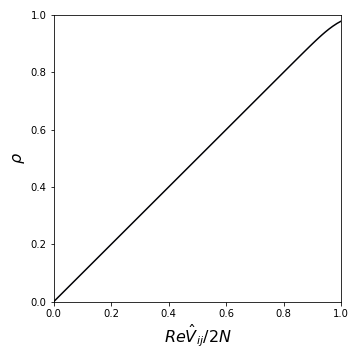
\includegraphics[width=80mm]{corrtestplot4.png}
\caption{The cross-correlation Van Vleck correction function (equation~\ref{crosscorr}) plotted with $\sigma_{x_1}=1.0, \sigma_{x_2}=1.0$.\label{corrplot}}
\end{figure}

\begin{figure}
\centering{}
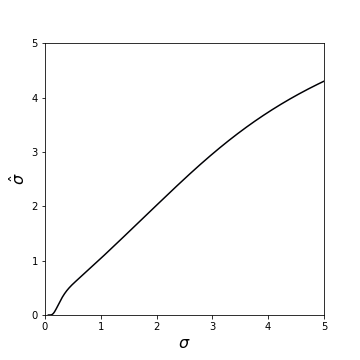
\includegraphics[width=80mm]{sigmatestplot4.png}
\caption{The auto-correlation Van Vleck correction function (equation~\ref{autocorr}).\label{sig}}
\end{figure}

\paragraph{}Equation \eqref{autocorr} is not invertible, so Newton's method for finding roots is used to iteratively solve the equation
\begin{equation}
0=\sqrt{\hat V_{11}/2N}-\left[7^2-\sum_{k=0}^6(2k+1)\textrm{erf}\left(\frac{k+0.5}{\sqrt{V_{11}/2N}\sqrt{2}}\right)\right]^{1/2}.
\end{equation}
A similar method was implemented for equation \eqref{crosscorr}. However, the correction algorithm has a high computational cost due to the $14^2$ exponential terms, which were each evaluated $\sim10$ times to compute the integral. By combining redundant terms, this number was reduced by a factor of 2. Though only $\sim5$ evaluations of equation \eqref{crosscorr} were required for the root-finding function to converge, the computation time remained prohibitively long at $\sim5$ hours per observation. To address this, an approximation using Chebychev polynomials was implemented which brings the correction time to $\sim30$ minutes per observation.

\paragraph{}
Equation \eqref{crosscorr} was fit to the following function
\begin{equation}\label{cheby}
\rho=c1 \cdot T_1(\kappa) + c3 \cdot T_3(\kappa) + c5 \cdot T_5(\kappa),
\end{equation}
where $T_k$ is the $k$th Chebyshev polynomial and $\kappa$ is either the real or imaginary part of $\hat V_{ij}/2N$. A two-dimensional grid of ($\sigma_{x_i}$, $\sigma_{x_j}$) was created, with values ranging between 0.9-4.5 and grid spacing 0.01. For each pair ($\sigma_{x_i}$, $\sigma_{x_j}$), a fitting function solved for the coefficients $c1, c3, c5$. These coefficients were saved and are imported into the Van Vleck correction function. For each crosscorrelation in the data, a bisection search finds the indices for the nearest $\sigma_{x_i}$ and $\sigma_{x_j}$ in the grid. A bilinear interpolation algorithm uses these indices to obtain the coefficients $c1$, $c3$, and $c5$. These coefficients are used in equation \eqref{cheby} to correct both the real and imaginary parts of $\hat V_{ij}/2N$.

\paragraph{}
A single MWA observation taken at 0.5 second time resolution and 40 kHz frequency resolution has $\sim10^{10}$ crosscorrelations. To apply a unique correction to each of these values in a time scale on the order of the time to read the files, the bilinear interpolation and Chebyshev evaluation stages were implemented in cython. This modification brought the correction time to $\sim30$ minutes in addition to the $\sim12$ minute read time.

\begin{figure}
\centering{}
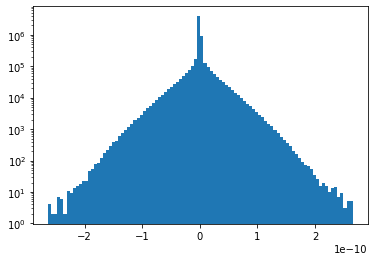
\includegraphics[width=80mm]{cheby_approx.png}
\caption{Differences between scaled crosscorrelations corrected using both an iterative integral solver and the Chebyshev approximation. These differences are on order $10^{-10}$, which is the scale at which the integral solver tests solutions. This suggests that using the Chebyshev approximation does not decrease the accuracy of solutions.\label{cheby_approx}}
\end{figure}

\paragraph{}
To check the Chebyshev polynomial approximation, a single timestamp of 2013 crosscorrelations was corrected both with an iterative integral solver and with the Chebyshev implementation. The differences between the resulting values are of order $10^{-10}$, as seen in figure \ref{cheby_approx}. As the iterative solver finds solutions that are accurate to $10^{-10}$, these differences indicate no change in accuracy in results obtained with the Chebyshev approximation.
%\paragraph{}
%The initial implementation of a Van Vleck correction for the MWA improves the artifacts of nonlinearity present in the data. However, residual artifacts prompt a deeper look into other quantization stages. In particular, the stage just before the 4 + 4 bit correlator quantization is implemented asymmetrically, so that positive and negative values are quantized differently. A second stage of the Van Vleck correction will address this asymmetric rounding.

\appendix
\section{Circular Complex Gaussian Random Variables}\label{ccrv}
\paragraph{}A circular complex random variable $Z=\Re(Z)+i\Im(Z)$ is defined as having a distribution that is invariant under a random phase shift:
\begin{align}
E[Z]&=E[e^{i\phi}Z]=0,\\
E[ZZ]&=E[e^{i\phi}Ze^{i\phi}Z],\\
E[ZZ^*]&=E[e^{i\phi}Ze^{-i\phi}Z^*]].
\end{align}
The last of these conditions is trivial. The first and second are only satisfied if $E[Z]=E[ZZ]=0$. Thus
\begin{align}
E[ZZ]&=0\\
&=E[(\Re(Z)+i\Im(Z))(\Re(Z)+i\Im(Z))]\\
&=E[\Re(Z)^2]-E[\Im(Z)^2]+iE[\Re(Z)\Im(Z)]+iE[\Im(Z)\Re(Z)]
\end{align}
and
\begin{align}
E[\Re(Z)^2]&=E[\Im(Z)^2],\\
E[\Re(Z)\Im(Z)]&=-E[\Im(Z)\Re(Z)]=0\label{CC1}.
\end{align}
For a complex random variable, the variance $\sigma_Z^2=E[ZZ^*]=E[\Re(Z)^2]+E[\Im(Z)^2]$. So in the case of a circularly complex random variable
\begin{equation}
\sigma_Z^2=2E[\Re(Z)^2]=2E[\Im(Z)^2].
\end{equation}
Two circular complex random variables sampled from the same distribution have the following relations
\begin{align}
E[\Re(Z_1)\Re(Z_2)]&=E[\Im(Z_1)\Im(Z_2)]\\
E[\Re(Z_1)\Im(Z_2)]&=-E[\Im(Z_1)\Re(Z_2)]\label{CC2}
\end{align}
If this relation does not hold for circular complex random variables sampled from different distributions, then some assumptions are required for the correlator input model.
\paragraph{}For example, consider the case of a correlator input $Z=S+N$, where $S$ and $N$ are both circular complex Gaussian random variables, that is, in addition to the conditions above, the real and imaginary parts of $S$ and $N$ are sampled from zero-mean Gaussian distributions. To treat $Z$ as circularly complex requires $E[\Re(Z)\Im(Z)]=0$. Thus
\begin{equation}
E[\Re(S)\Im(S)]+E[\Re(N)\Im(N)]+E[\Re(S)\Im(N)]+E[\Re(N)\Im(S)]=0.
\end{equation}
The first two terms vanish according to \eqref{CC1}. If \eqref{CC2} applies to circular complex random variables sampled from different distributions, the last two terms vanish. If the relation does not apply, then it is required that $E[\Re(S)\Im(N)]=E[\Re(N)\Im(S)]=0$, that is, that the sky signal and receiver noise are uncorrelated. 
\nocite{*}
\printbibliography
%\bibliographystyle{apsrmp4-2}
\end{document}